\documentclass{report}
\usepackage{cite}
\usepackage{titlesec}
\usepackage{amsmath}
\usepackage[english]{babel}
\usepackage{caption}
\usepackage{multirow}
\usepackage{tikz}
\usepackage{amsmath}
\usepackage{amssymb}
\usetikzlibrary{calc}
\usetikzlibrary{arrows}
\usepackage{pgfplots}
\captionsetup[figure]{font=small}	
\captionsetup[table]{font=footnotesize}
\newcommand{\R}{\mathbb{R}}
\usepackage{float}
\tolerance=1
\emergencystretch=\maxdimen
\hyphenpenalty=10000
\hbadness=10000
\usepackage{array}
\usepackage{textgreek}
\usepackage{graphicx}
\graphicspath{ {./images/} }

\begin{document}


\begin{titlepage}
\begin{center}
\vspace*{0.8cm}
\begin{figure}[H]
\centering

\includegraphics[width=0.4\textwidth]{logo_uni}
\end{figure}
\LARGE{\textsc{University of Padua}}\\
\vspace*{0.1cm}
\Large{\textsc{Department of Information Engineering}}\\
\vspace*{1.0cm}
\Large{\textsc{Information Security Report}}\\
\vspace*{0.1cm}
\Large{\textsc{Laboratory Session 2}}\\
\vspace*{0.8cm}
\huge{\textbf{Implementation of random binning encoding and secrecy rate
evaluation}}\\
\vspace*{1cm}
\end{center}
\large{\textit{Author:}}
\hfill
\large{\textit{Teacher:}} \\
\large{ZANON \textsc{ALBERTO}}
\hfill
\large{Nicola \textsc{Laurenti}}\\
\large{MICHELON \textsc{LUCA}}\\
\large{SCREMIN\textsc{ NICOLA}}\\
\large{NIKHIL \textsc{KARAKUCHI CHIDANANDA }}\\
\large{PORRO \textsc{THOMAS}}\\

\vspace*{0cm}
\begin{center}
\large{29 November 2020}\\
\end{center}
\end{titlepage}
\pagebreak


\setcounter{page}{1}
\pagenumbering{arabic}
\chapter*{Solution}
Our solution to laboratory 2 is entirely implemented using Python. Specifically, we made use of the {\tt NumPy} library to easily manipulate vectors and quickly compute operations between them. The solution is composed of 8 Python source files: {\tt main.py} contains all the function for tasks, {\tt task1.py} contains functions necessary to carry out the implement the wiretap channel, so that it accepts an
input  and produces the corresponding pair of outputs (y; z), {\tt task2.py} contains random encoder function to implement the random binning encoder, so that it accepts an input and produces the corresponding output, {\tt task3.py} contain random decoder function to implement the legitimate decoder, so that it accepts an input and produces the corresponding output,  {\tt task4.py} contains the functions implement the encoder + eavesdropper channel, {\tt task5.py}  contains function to implement the wiretap BSC, {\tt task6.py} contains functions for repeat the simulations in Tasks 3-4 with the wiretap BSC, evaluate the resulting reliability in terms of Bob's error rate on the secret message chain P, evaluate the resulting the secrecy in terms of leaked information to Eve on the secret message I and compute an upper bound to the mechanism security in terms of distinguishability from the ideal
counterpart and {\tt utils.py} contains function to convert the string to array and the array to string. 
 \section*{Task 1}
We implemented the uniform error channel using the function {\tt legittimate\_channel(x)} the legitimate channel introduces at most 1 binary error per word,
 Legitimate a random integer for choosing which is the error and XOR with the the input and {BitArray(bin=errors[index]).uint} transforms binary string to integer. and {\tt eve\_channel(x)} for the eavesdropper channel introduces at most 3 binary error per word, and the {\tt main()} function contains the variables  x = "01001000"
  y = []
  z = []
  contyz = 0
  conty = 0
  contz = 0
  n = 25000 after that we call the function  {\tt legittimate\_channel(x)} and adds new word to a list y.append(word\_y) and Same for Eve by  calling {\tt eve\_channel(x)} after the all list is appended we Verify the conditional independence and uniformity and print the output and plot the graphic for Legitimate channel and plot the graphic for Eavesdropper channel.  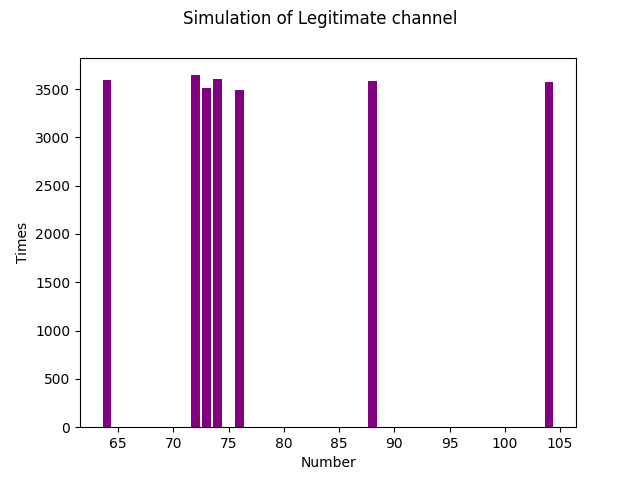
\includegraphics[width=10cm,height=7cm]{Figure_1} \linebreak
 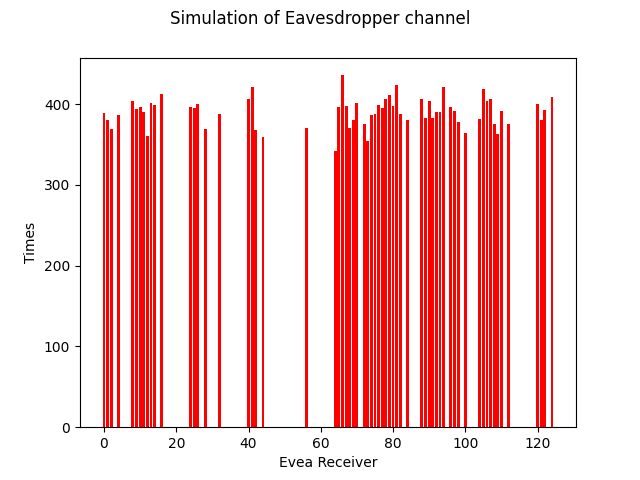
\includegraphics[width=10cm,height=7cm]{Figure_2}
  \section*{Task 2}
  In task 2 we are using the random lib for Generate pseudo-random numbers and BitArray lib for efficient arrays of booleans for better implementation, we defined X array variable for storing the codewords, and {\tt rand\_encoder(d)} function for Implement the random binning encoder, first we checks which codeword starts with the prefix and gets it and Calculates the complement of the binary given as input and the codeword x is chosen randomly and uniformly within the bin associated to the message u, to optimise the code we could compute the complement if, and only if, the rand == 1, in this i preferred to show the two choices and how the randomness choice it.
\section*{Task 3}

\section*{Task 4}

\section*{Task 5}

\section*{Task 6}



\end{document}

